\documentclass[10pt,twocolumn,letterpaper]{article}

\usepackage{statcourse}
\usepackage{times}
\usepackage{epsfig}
\usepackage{graphicx}
\usepackage{amsmath}
\usepackage{amssymb}

% Include other packages here, before hyperref.

% If you comment hyperref and then uncomment it, you should delete
% egpaper.aux before re-running latex.  (Or just hit 'q' on the first latex
% run, let it finish, and you should be clear).
\usepackage[breaklinks=true,bookmarks=false]{hyperref}


\statcoursefinalcopy


\setcounter{page}{1}
\begin{document}


%%%%%%%%%%%%%%%%%%%%%%%%%%%%%%%%%%%%%%%%%%%%%%%%%%%%%%%%%%%%%%%
% DO NOT EDIT ANYTHING ABOVE THIS LINE
% EXCEPT IF YOU LIKE TO USE ADDITIONAL PACKAGES
%%%%%%%%%%%%%%%%%%%%%%%%%%%%%%%%%%%%%%%%%%%%%%%%%%%%%%%%%%%%%%%



%%%%%%%%% TITLE
\title{\LaTeX\ Template for NLP Final Project Report}

\author{Tom Arend\\
{\tt\small t.arend@phd.hertie-school.org}
\and
Nicolai Berk\\
{\tt\small nicolai.berk@gmail.com}
}

\maketitle
%\thispagestyle{empty}


% MAIN ARTICLE GOES BELOW
%%%%%%%%%%%%%%%%%%%%%%%%%%%%%%%%%%%%%%%%%%%%%%%%%%%%%%%%%%%%%%%

%%%%%%%%% ABSTRACT
\begin{abstract}
   The measurement of ideology is one of the major applications of text analysis in political science. However, researchers often face scarcity of available labelled data to train supervised models for their specific domain. Manual annotation is costly and often severely affected by subjective bias. We propose to fine-tune transformer models on available, labelled political texts issued by political parties to obtain a classifier of political ideology. Using a unique dataset of newspaper articles authored by politicians, we test such an application in the German context. Comparing transformer neural networks fine-tuned on different data sets of party press releases, we present evidence on the feasibility of such an approach. This contributes to the broad literature on text analysis in the political domain, informing researchers on the limitations of training powerful deep learning models on political language with scarce training data. The experiments conducted by the authors indicate that the training on party labels cannot be easily translated to the domain of newspaper articles but that supervised models are highly sensitive to minor changes in the inputs. It is thus recommended to refrain from using deep learning in the absence of sufficient training data\footnote{GitHub repository: \url{https://github.com/nicolaiberk/nlpdl\_project}}.
\end{abstract}


% \begin{itemize}
% {\color{blue}

% \item Your final report should be written in the same style as an NLP research paper, and ideally written in a way that a fellow NLP student could understand. It should be a PDF created using this template.

% \item Your report should be {\bf 8 pages} (not including references).

% \item You must include a link to your GitHub repository for the project as the first footnote on the first page. \footnote{Here's a link to my GitHub account: \url{https://github.com/sjankin} and Hannah's \url{https://github.com/hannahbechara}. Make sure that your repository is accessible to us!}

% \item As a reminder, the midterm report template included links to resources to help you improve your technical writing. You can use these, and previous feedback you've received, to improve your technical writing.

% \item Your final project report will be graded holistically, taking into account many criteria: originality, performance of your methods, complexity of the techniques you used, thoroughness of your evaluation, amount of work put into the project, analysis quality, writeup quality, demonstrating strong understanding, etc. You will also receive some brief feedback on your report. 

% \item All final reports will be posted on the course website as a blogpost and presentation recording.

% \item Your final report should contain the following sections (though you can use a different structure if you prefer). Sections with an asterisk (*) were \emph{not} part of the milestone.

% }
% \end{itemize}

%%%%%%%%% BODY TEXT
\section*{Introduction}

% The introduction explains the problem, why it's difficult, interesting, or important, how and why current methods succeed/fail at the problem, and explains the key ideas of your approach and results. Though an introduction covers similar material as an abstract, the introduction gives more space for motivation, detail, references to existing work, and to capture the reader's interest.

The measurement of ideology and political bias\footnote{'Political bias', 'ideological slant' and variations of the two are used interchangeably in this report.} are the subject of much research on political texts \cite{Bilbao-Jayo2018, Laver2003, Simoes2020}. Despite significant advances in our understanding and detection of ideology, most researchers still face significant constraints when working with text. Notably, they face a lack of appropriately labelled training data for supervised learning. This is linked to the high costs incurred by manually annotating a significant number of speeches, texts, or sentences. Often, the detection of ideological bias might be highly dependent on the coders' subjective assessment. Instead, researchers could train models on other sources of text with clear and available labels and subsequently apply them to the desired texts using transfer learning.

We conduct experiments with differently fine-tuned deep learning models to understand if and how transfer learning can be used to measure bias in the absence of abundant training data. We fine-tune a deep neural network to predict the authoring political party of German press releases. Once the model is fine-tuned to predict the authoring party of press releases, it is applied to estimate the bias of newspaper. In addition, we compare this approach to models that are (additionally) fine-tuned in the domain of newspaper articles to assess the effectiveness of this alternative fine-tuning process. While the application of transformers to measure bias is not entirely new in political science \cite{Vig2020}, we want to move beyond the current state-of-the-art by measuring the precise implications of different fine-tuning procedures. 

Beyond testing the effectiveness of this two-step fine-tuning process, this project seeks to develop a state-of-the-art deep learning model for the measurement of political bias in newspaper articles.  Newspapers represent an important institution in the political world, affecting phenomena ranging from polarization to voter turnout. Much like the shadows in Plato's allegory of the cave, news provide elites and citizens with a representation of a reality they are not able to see themselves \cite{Plato520a}. The media have the power to affect voting behaviour \cite{Chiang2011, Ladd2009}, as well as polarise the electorate \cite{Lelkes2017} or motivate them to turn out to vote \cite{Gentzkow2010}. 

Given this importance of the news media for the study of politics, it is surprising that few papers deploy state-of-the-art deep learning technologies to classify ideological bias in news articles. Gentzkow and Shapiro estimate slant in US newspapers by identifying bi- and trigrams' indicative of a congressional speakers' party, and apply the resulting dictionary to newspapers to scale them \cite{Gentzkow2010}. More recently, Widmer et al. have assessed polarisation in the US media environment using a supervised model. They train a classifier on bigrams, predicting whether content was produced by a left-leaning network (CNN) or a right-leaning network (Fox news) \cite{Widmer2020}. We believe both approaches are likely inferior to more complex deep learning models, as such novel approach would not incorporate idiosyncratic phrases used by the specific networks identified to train the data. Using party labels to train classifiers is more straightforward, as it places newspapers within the existing context. If existing approaches to classify newspaper slant can be improved upon, or even just complemented, we could provide an additional tool for researchers to study drivers and effects of media bias. A working state-of-the-art model might even renew interest in the subject matter and encourage researchers to find new and exciting applications for it. 

Outside of academia, a confident and robust classifier of newspaper bias might help readers to identify when they are reading an article that is overly partisan. This would perhaps encourage them to approach certain news sources with more scepticism and hold news outlets to higher editorial standards. In the long run, the highlighting of biases in articles might counteract the worrying polarization of entire electorates.

The experiments conducted by the authors indicate that the training on party labels cannot be easily translated to the domain of newspaper articles. While our models show impressive performance in validation, out-of-sample test sets, and even when crucial information like the party names are censored in the training data, this does not translate into stable estimates of newspaper bias. While the broad expectations of newspapers' left-right placement are always confirmed, the estimates about which specific party a newspaper resembles are highly sensitive to minor changes in the inputs. It is thus recommended to refrain from using deep learning in the absence of sufficient training data.\\

\section*{Related Work}

% This section helps the reader understand the research context of your work, by providing an overview of existing work in the area.

% \begin{itemize}

% \item You might discuss: papers that inspired your approach, papers that you use as baselines, papers proposing alternative approaches to the problem, papers applying your methods to different tasks, etc.

% \item This section shouldn't go into deep detail in any one paper (for example, there probably shouldn't be any equations) -- instead it should explain how the papers relate to each other, and how they relate to your work.

% \end{itemize}

Measuring ideology is the prime use-case of automated text analysis in political science. While some work has used supervised learning to understand political polarisation \cite{Ash2017} as well as media slant \cite{Widmer2020}, this existing work estimates the polarisation of political actors or newspapers across time, or simply the similarity of one news source to others. Existing models have for the most part relied on bag-of-words approaches, including the scaling of texts using supervised \cite{Laver2003} or unsupervised models \cite{Slapin2008}. Unsurprisingly, the performance of these models has so far proven unreliable, lagging behind the accuracy of human coders or expert judgement \cite{Brauninger2013, Hjorth2015, Koljonen2020}. Recent applications have assessed the ability of deep learning models to replicate human coding of party manifestos \cite{Bilbao-Jayo2018} or estimate ideology directly using supervised classification \cite{Simoes2020}. These applications employ RNNs or CNNs. We feel they could be improved upon with state-of-the-art transformer neural networks.

Much less work has been devoted to the measurement of the ideological leaning of newspapers. While some work has assessed the impact of endorsements of specific candidates \cite{Chiang2011, Ladd2009}, there have been few attempts to scale newspapers on ideology. Gentzkow and Shapiro estimate slant in US newspapers by identifying bi- and trigrams' indicative of a congressional speakers' party, and apply the resulting dictionary to newspapers to scale them \cite{Gentzkow2010}. More recently, Widmer et al. have assessed polarisation in the US media environment using a supervised model. They train a classifier on bigrams, predicting whether content was produced by a left-leaning network (CNN) or a right-leaning network (Fox news) \cite{Widmer2020}.

We believe both approaches are likely inferior to more complex deep learning models, as such novel approach would not incorporate idiosyncratic phrases used by the specific networks identified to train the data. Using party labels to train classifiers is more straightforward, as it places newspapers within the existing context. However, any algorithm trained on a different dataset than applied to must be subject to careful validation.

In this project, we provide such validation. % jadajadajada, surprisingly our evidence indicates that it is not straightforward to apply deep-learning models trained on party labels....

\textbf{[ADD ASH ET AL PAPER ON TRANSFER LEARNING]}

\section*{Proposed Method}

% This section details your approach(es) to the problem. For example, this is where you describe the architecture of your model, and any other key methods or algorithms.

% \begin{itemize}

% \item You should be specific when describing your main approaches -- you probably want to include equations and figures.
% \item You should also describe your baseline(s). Depending on space constraints, and how standard your baseline is, you might do this in detail, or simply refer the reader to some other paper for the details. 
% \item If any part of your approach is original, make it clear (so we can give you credit!). For models and techniques that aren't yours, provide references.
% \item If you're using any code that you didn't write yourself, make it clear and provide a reference or link. When describing something you coded yourself, make it clear (so we can give you credit!).

% \end{itemize}

We propose the use of transfer learning to identify newspaper slant: a pre-trained transformers model is fine-tuned to identify the authoring party of press releases. Then, this model is applied to a range of newspaper articles, indicating which parties' communication an article most resembles. This approach is useful, as political parties represent the major organisers of and reference points for political ideology. More importantly, party-issued political texts constitute data that already carry ideological labels and need no further labour for annotation. It therefor represents an efficient and broadly available source of data for transfer learning to identify ideological bias in newspaper articles. 'Bias' is here defined as the similarity of a set of text to a given party's communication. This is a reasonable definition, as political parties constitute the major points of reference and organizers of ideology in contemporary democracies. 

In detail, we employ pre-trained BERT neural network models for German language\footnote{Link to the model page: \url{https://huggingface.co/transformers/model_doc/distilbert.html}} and compare how three different training processes affect model performance. We expect optimal performance from a transformer neural network that was fine-tuned in two steps. First we use the pre-trained model to classify party press releases by issuing party. Secondly, the model is applied in its actual domain to estimate ideological bias in news articles. We fine-tune and subsequently validate the model using op-eds by politicians. These unique data have the advantage of carrying party labels, allowing a direct transfer of the categories from the initial fine-tuning process (first step) to the outcome of interest. We compare this fine-tuned model to a BERT model that was not fine-tuned on party press releases and one that was not fine-tuned on newspaper data. This leaves us with three models:

\begin{enumerate}
    \item A model only fine-tuned on newspaper articles authored by politicians.
    \item A model only fine-tuned on party press releases.
    \item A model both fine-tuned on press releases and politicians' newspaper contributions.
\end{enumerate}

This approach allows to assess by how much model performance is improved upon, when including information from both party press releases and newspaper data. This is especially useful as it allows us to comparatively assess the performance of a model that has never seen data from the domain of interest (model 2). If this model performs well, this constitutes strong evidence that party communication can be used to train classifiers which are applied in a diverse set of domains with scarce or no training data. If model 3 severely outperformed model 1, this would corroborate the idea that information from available sets of texts from political actors can be used to improve ideology measurements for other sets of text.  \\

\textbf{[ADD DISCUSSION OF CHANGES IN RESPONSE TO MIDTERM FEEDBACK]}\\

\textbf{[ADD DISCUSSION OF BERT; BERT OPTIMISATION \& LSTM]}

\section{Experiments}

% This section contains the following.

\paragraph{Data:} In this project, we planned to use four distinct data sources:\\
\begin{itemize}
    \item A dataset of over 40,000 German party press releases issued between 2010 and 2019, collected by the SCRIPTS project\footnote{\url{https://www.scripts-berlin.eu/index.html}. Special thanks go to Lukas Stötzer for the effortless (for us) provision of the data.}.
    \item A collection of over 2 million German newspaper articles from six major newspapers, published between 2013 and 2019, collected by one of the authors in a previous project (\cite{Krause2021}).
    \item A set of German newspaper articles authored by politicians collected as part of this project.
    \item A survey of newspaper readers asking them about the partisan bias of their newspaper, to generate a first indication of the expected results (\textbf{CITE GLES}).
\end{itemize}
% Describe the dataset(s) you are using (provide references). If it's not already clear, make sure the associated task is clearly described.


\paragraph{Software}: All software for this project was self-written. However, we relied on the programming languages R and Python \textbf{[INSERT REFERENCES]}, as well as corresponding packages, most importantly Huggingface's \texttt{transfomers} package and \texttt{pytorch} for the training of our models.

% Briefly list (and cite) software software you used.

% \paragraph{Hardware}: If relevant, list hardware resources you used.

\paragraph{Evaluation method:}  So far, we have successfully fine-tuned a BERT-model to classify party-press releases by authorship (model 2, serving as the basis for model 3). The performance of this model is shown in \ref{fig:party}. As the reader can see, the model performs at a very high, near-perfect level. We believe that the classification performance made hyper-parameter optimisation at this stage somewhat obsolete. It might however be useful in the second stage of fine-tuning. The impressive performance of this model on the press releases was rather surprising to the authors and shifted the initial focus of the project away from improving the classification of party press releases to the comparison of improvements in the two-step fine-tuning process. \\

\begin{figure}
    \centering
    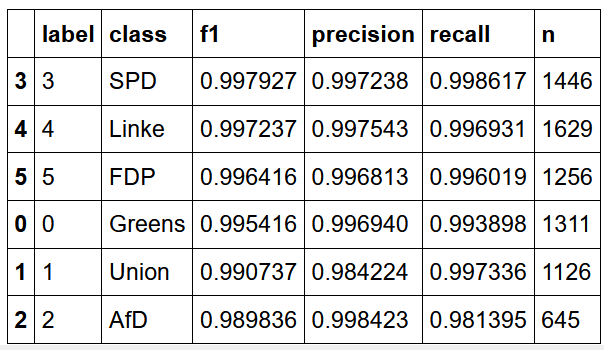
\includegraphics[width=0.4\textwidth]{reports/midterm-report-latex/figures/party_class.png}
    \caption{Performance of default BERT model for the classification of party press releases.}
    \label{fig:party}
\end{figure}

For the final assessment of classifier performance, we will use a unique, newly collected set of politicians' op-eds and interviews. This data enables us to compare the impact of different fine-tuning processes (using party press releases, newspaper articles, or both) on model performance, as the outcome categories (authorship party) are identical. We aim for a balance of precision and recall, and will therefore evaluate the models' F1-scores. Additionally, we will assess generalisability by assessing the placement of newspapers based on estimates for all news articles. Left-wing newspapers such as the TAZ should be placed closer to left-wing parties (Grüne, SPD, Linke) than right-wing newspapers (FAZ, WELT).

\textbf{[DESCRIBE HOW MODELS PERFORM IN OUT-OF-DATA-SAMPLE AND PARTY LABEL REMOVAL]}


\textbf{[DESCRIBE PROCESS OF EVALUATION SINCE MIDTERM; AS WELL AS SURVEYDATA]}

\paragraph{Experimental details:}In total, we train three different models on three different forms of input data. We use the 'distilbert-base-german-cased' model from the Huggingface transformer library\footnote{\url{https://huggingface.co/bert-base-german-cased}.} as a baseline. This deep-learning model has been trained to efficiently solve different classification tasks on 12 GB of German language data, including Wikipedia, legal data, and news. We decided on three training epochs, a training batch size of 16, and a weight decay of $0.01$ for regularisation. This might change in the future, depending on the model's performance on the newspaper articles. The configuration of our hyper-parameters hence largely follows the defaults and is as follows\footnote{The model's default settings can be found here: \url{https://huggingface.co/distilbert-base-german-cased/blob/main/config.json}.}:

\begin{itemize}
    \item Training epochs: $3$
    \item Training batch size: $16$
    \item We apply a weight decay as a form of regularisation: $0.01$
    \item Maximum sequence length (longer articles were truncated): $512$
    \item Dropout for each layer: $10\%$
\end{itemize}

\textbf{[OPTIMISED BERT]}

\textbf{[LSTM]}


% How you ran your experiments (e.g. model configurations, learning rate, training time, etc.)


\paragraph{Results:} We classified a training set of 4,000 newspaper articles using model 2 (fine-tuned on party press releases). We expected articles from conservative newspapers FAZ and Welt to be more similar to Union and FDP and possibly the AfD, especially compared to the progressive TAZ. Spiegel Online (SPON) is expected to be equally similar to right- and leftwing newspapers.

For the three daily newspapers, we can validate our expectation using survey data from the 2017 German Longitudinal Election Study's Rolling Cross-Section (GLES-RCS; \cite{GLES2017RCS}). The study asked respondents whether they read a daily newspaper, and if so, whether they felt the newspaper's reporting favored certain parties over others. While these estimates are likely biased by the respondents own political stances (and as such likely underestimate the ideological extremity of their paper), they do provide a first clue. Table \ref{tab:gles} shows the aggregated results of this question. We can see that - in line with our initial expectation, FAZ and Welt are placed close to the centre-right Union and FDP (but also SPD), while the more left-wing TAZ is placed close to the three centre-left and left parties (Linke, Grüne, SPD; but note that this estimate is based on only 89 respondents). Note that none of the newspapers is considered to report favorable for the AfD.

\begin{table}[!htbp] \centering 
    \begin{tabular}{@{\extracolsep{0pt}} lccccccc} 
    \\[-1.8ex]\hline 
    \hline \\[-1.8ex] 
    Paper &  Linke & Grüne & SPD & Union & FDP & AfD & N \\ 
    \hline \\[-1.8ex] 
    % bild & $0.01$ & $0.01$ & $0.14$ & $0.36$ & $0.04$ & $0.01$ & $796$ \\ 
    FAZ & $0.01$ & $0.02$ & $0.11$ & $0.33$ & $0.11$ & $0$ & $390$ \\ 
    % SZ & $0.02$ & $0.04$ & $0.19$ & $0.20$ & $0.03$ & $0$ & $458$ \\ 
    TAZ & $0.23$ & $0.24$ & $0.27$ & $0.16$ & $0.04$ & $0$ & $89$ \\ 
    Welt & $0.01$ & $0.02$ & $0.18$ & $0.35$ & $0.09$ & $0.03$ & $209$ \\ 
    \hline \\[-1.8ex] 
    \end{tabular} 
  \caption{Validation reference: readers' assessment of newspapers' bias} 
  \label{tab:gles} 
\end{table} 

We estimated the similarity of reporting by German newspapers FAZ, Spiegel, TAZ and Welt using the simple BERT model, given its outstanding performance on the training data. The results can be seen in table \ref{tbl:means}, which shows the average probability for an article to be classified as being authored by a given party. As expected, FAZ and Welt are very similar to Union (81\%) and FDP (58\%/55\%), but also rather similar to the Greens (36\%/35\%). While they show the highest similarity to the AfD (8\%/7\%), similarity to the radical-right party is generally on a very low level among all newspapers. Spiegel Online (SPON) shows lower similarity to the FDP and closer to Union and Greens, but is generally rather similar to the right-wing newspapers. As expected, the TAZ shows a comparatively different profile, being very similar to the Greens (average likelihood 70\%), and less similar to the Union parties (41\%), the FDP (32\%), and the AfD (5\%). Surprisingly, it also shows the lowest similarity to the Linke (13\%). Maybe most surprising is the general low similarity to SPD press releases (4\%/5\%). It seems the party has a rather distinctive style in its press releases.\\

\begin{table}[!htbp] \centering 
    \begin{tabular}{@{\extracolsep{1pt}} lcccccc}
    \\[-1.8ex]\hline 
    \hline \\[-1.8ex] 
    Paper & Linke & Grüne & SPD & Union & FDP & AfD \\ 
    \hline \\[-1.8ex] 
    FAZ & $0.15$ & $0.36$ & $0.05$ & $0.81$ & $0.58$ & $0.08$ \\ 
    Spiegel & $0.11$ & $0.39$ & $0.05$ & $0.89$ & $0.34$ & $0.07$ \\ 
    TAZ & $0.13$ & $0.69$ & $0.04$ & $0.41$ & $0.32$ & $0.05$ \\ 
    Welt & $0.15$ & $0.35$ & $0.05$ & $0.81$ & $0.55$ & $0.07$ \\ 
    \hline \\[-1.8ex] 
    \end{tabular} 
  \caption{Mean similarity estimate to each party by newspaper, based on training data including party labels and large time frame.} 
  \label{tbl:means} 
\end{table}

We restricted the time-frame of the training time, which severely affected our results: 

\begin{table}[!htbp] \centering 
  \caption{Placement of newspapers with date-restricted, labelled training data.} 
  \label{} 
\begin{tabular}{@{\extracolsep{1pt}} lccccccc} 
\\[-1.8ex]\hline 
\hline \\[-1.8ex] 
Paper & Linke & Grüne & SPD & Union & FDP & AfD \\ 
\hline \\[-1.8ex] 
FAZ & $0.20$ & $0.20$ & $0.26$ & $0.19$ & $0.85$ & $0.40$ \\ 
Spiegel & $0.13$ & $0.17$ & $0.23$ & $0.07$ & $0.94$ & $0.16$ \\ 
TAZ & $0.22$ & $0.11$ & $0.67$ & $0.20$ & $0.49$ & $0.29$ \\ 
Welt & $0.20$ & $0.15$ & $0.26$ & $0.24$ & $0.84$ & $0.37$ \\ 
\hline \\[-1.8ex] 
\end{tabular} 
\end{table} 
Additionally censoring party labels in the training data:

\begin{table}[!htbp] \centering 
  \caption{Placement of newspapers with removed party labels.} 
  \label{} 
\begin{tabular}{@{\extracolsep{1pt}} lccccccc} 
\\[-1.8ex]\hline 
\hline \\[-1.8ex] 
Paper & Linke & Grüne & SPD & Union & FDP & AfD \\ 
\hline \\[-1.8ex] 
FAZ & $0.15$ & $0.36$ & $0.05$ & $0.81$ & $0.58$ & $0.08$ \\ 
Spiegel & $0.11$ & $0.39$ & $0.05$ & $0.89$ & $0.34$ & $0.07$ \\ 
TAZ & $0.13$ & $0.69$ & $0.04$ & $0.41$ & $0.32$ & $0.05$ \\ 
Welt & $0.15$ & $0.35$ & $0.05$ & $0.81$ & $0.55$ & $0.07$ \\ 
\hline \\[-1.8ex] 
\end{tabular} 
\end{table}


\textbf{[if time: COMPARE TO LSTM, OPTIMISED BERT}
% Report the quantitative results that you have found so far. Use a table or plot to compare multiple results and compare against baselines.

\paragraph{Comment on your quantitative results.} \textbf{[WHAT DOES THIS MEAN? IS THERE A MODEL THAT IS CONVINCING? WHAT IS GOING ON? - LETS DISCUSS THIS ONCE THE LSTM AND OPTIMISED BERT RESULTS ARE IN]}
% Are they what you expected? Better than you expected? Worse than you expected? Why do you think that is? What does this tell you about what you should do next? Including training curves might be useful to discuss whether things are training effectively.

\section{*Analysis}

% Your report should include some qualitative evaluation. That is, try to understand your system (how it works, when it succeeds and when it fails) by measuring or inspecting key characteristics or outputs of your model.

% \begin{itemize}
% \item Types of qualitative evaluation include: commenting on selected examples, error analysis, measuring the performance metric for certain subsets of the data, ablation studies, comparing the behaviors of two systems beyond just the performance metric, and visualizing attention distributions or other activation heatmaps.

% \item The Practical Tips lecture notes has a detailed section on qualitative evaluation -- you may find it useful to reread it.
% \end{itemize}

\textbf{[DISCUSS WHETHER IMPROVED MODELS ARE EXPECTED TO SOLVE THIS PROBLEM]}


\section{*Conclusions}
% Summarize the main findings of your project, and what you have learnt. Highlight your achievements, and note the primary limitations of your work. If you like, you can describe avenues for future work.

\section{Acknowledgements}

We thank the vast community contributing to the development of machine learning tools, specifically huggingface. Additionally, we want to thank Lukas Stötzer for provision of the training data and Hauke Licht for providing us with a first notebook.

% List acknowledgements if any. For example, if someone provided you a dataset, or you used someone else's resources, this is a good place to acknowledge the help or support you received.

\section{Contributions}

Describe the contributions of each team member who worked on this project. You should write a brief summary of what each team member did for the project (about 1 or 2 sentences per person). We will read these descriptions and cross-reference with GitHub contributions in your project repository. For almost all teams, it will have no effect (team members all receive same grade), but for teams with very unequal contribution, we may investigate and/or give different grades to team members.

\section{References}
% Your references section should be produced using BibTeX.
{\small
\bibliographystyle{ieee}
\bibliography{bibliography.bib}
}

\section{*Appendix}
If you wish, you can include an appendix, which should be part of the main PDF, and does not count towards the 8 page limit. Appendices can be useful to supply extra details, examples, figures, results, visualizations, etc., that you couldn't fit into the main paper. However, your grader does not have to read your appendix, and you should assume that you will be graded based on the content of the main part of your paper only.


\end{document}
